\documentclass{report}

% packages
\usepackage[utf8]{inputenc}
\usepackage{amsthm}
\usepackage{amsmath}
\usepackage{amssymb}
\usepackage{enumerate}
\usepackage{graphicx}
\usepackage[margin=1.4in]{geometry}

\usepackage{calrsfs}
\DeclareMathAlphabet{\pazocal}{OMS}{zplm}{m}{n}

% definitions and commands
\newtheorem{theorem}{Theorem}
\newtheorem{lemma}{Lemma}
\newtheorem{corollary}{Corollary}
\newtheorem{remark}{Remark}
\newtheorem{proposition}{Proposition}
\newtheorem{definition}{Definition}

\newcommand{\norm}[1]{\left\lVert#1\right\rVert}
\newcommand{\polylog}{\: \mathrm{polylog} \:}

\title{Expected Recourse of Incremental Cycle Detection Algorithms}
\author{Martin Costa}
\date{August 2020}

\begin{document}

\maketitle

\chapter{Expected Recourse Bounds for Trees under Adversarial Arrival}

\section{My Results}

While working on the conjectures that the simple algorithms are expected to have low total recourse under random order arrival, I discovered many interesting properties of the one-way search algorithm $\pazocal A_1$. While I was not able to prove the conjecture that I initially set out to prove, I was able to use the properties that I found to prove that by randomising the initial ordering before running $\pazocal A_1$ we obtain low expected total recourse under \textit{adversarial} arrival on trees.\footnote{Alternatively, we can interpret this result as saying that we can construct a \textit{randomized algorithm} which has low expected total recourse on all trees}

This chapter will be devoted to constructing a framework which I will then use to prove this fact. More formally, I will be proving the following Theorem

\begin{theorem}
Let $\pazocal T = (V,E)$ be a tree and $\pazocal E$ be any insertion sequence of $\pazocal T$, then
\[ \mathbb{E}_{\prec \in \mathcal S_V}[ rec(\pazocal E, \prec)] = \pazocal{O}(n\log n) \]
\end{theorem}

As an immediate corollary of this Theorem we get a weaker version of the conjecture I set out to prove, which is that there exists an algorithm with low expected total recourse under \textit{random order} arrival on trees. More formally

\begin{corollary}
Let $\pazocal T = (V,E)$ be a tree, then
\[ \mathbb{E}_{\prec \in \mathcal S_V, \pazocal E \in \mathcal S_E}[ rec(\pazocal E, \prec)] = \pazocal{O}(n\log n) \]
\end{corollary}

% CHAPTER 1
\section{Properties of $\pazocal A_1$}

I will start off my going over some of the properties of the one-way search algorithm $\pazocal A_1$. We assume from now on that $\pazocal{A}$ always performs forward searches. For the rest of this section fix DAG $G=(V,E)$.

\begin{definition}
At some point during the run of $\pazocal A_1$ on $G$ for some insertion sequence and initial ordering, we say an edge $(u,v)$ is \textbf{critical} to $w$ if its insertion would increase the amount of nodes that can reach $w$. Similarly, we say that an edge $(u,v)$ is \textbf{right critical} to $w$ if its insertion would cause the recourse of $w$ to increase. We say $u$ is (right) critical to $w$ if there exists an edge $(u,v)$ that is (right) critical to $w$.
\end{definition}

This definition has the following obvious properties.

\begin{proposition}
During the run of $\pazocal{A}$ on $G$, the insertion of an edge $(u,v)$ can only increase the recourse of $w$ if $(u,v)$ is critical to $w$, i.e. all right critical edges (and nodes) to $w$ are also critical to $w$.
\end{proposition}

\begin{proposition}
Given any $u,v \in V$, if $u$ is \textbf{not} an ancestor of $v$ in $G$, then $u$ can never be critical to $v$ during the run of $\pazocal{A}$ on $G$. 
\end{proposition}

Combining these two properties we get the following.

\begin{lemma}
Fix an insertion sequence and an initial ordering for $G$, and use these to induce an insertion sequence and an initial ordering for $H = G[reach^{-1}_{G}(x)]$ for some node $x$. Then given some $u \in reach^{-1}_{G}(x)$, the recourse of $u$ in the run of $\pazocal A_1$ on $G$ equals the recourse of $u$ in the run of $\pazocal A_1$ on $H$.
\end{lemma}

\begin{proof}
Let $E^* = E(G) \setminus E(H)$. We want to show that the relative ordering of the nodes in $V(H)$ cannot be affected by the insertion of edges in $E^*$ and only depends on the order of insertions of the edges in $E(H)$ and not on $E^*$.

By the propositions above, we can see that the insertion of an edge $(u,v)$ can only cause the recourse of some node $w$ to increase if $v$ can reach $w$. Suppose that the insertion of some $e = (u,v) \in E^*$ causes the recourse of $w \in V(H)$ to increase. Then we get that $u,v \in V(H)$, so $e \in E(H)$, giving us a contradiction.

Suppose we insertion some $e = (u,v) \in E(H)$ into the graph. The algorithm decides which nodes to move by performing a one-way search starting from $v$, and moves them in such a way that the relative ordering of all nodes that are moved is preserved. Since the presence of any edges from $E^*$ in the graph cannot change the nodes in $V(H)$ that the search is able to find, we can deduce that their presence in the graph will not change the effect of the algorithm on the relative ordering of the nodes in $V(H)$, and that this will depend purely on the state of the ordering and which edges from $E(H)$ had already been inserted right before the insertion occurred.
\end{proof}

Intuitively, this lemma is saying that the effect of $\pazocal A_1$ on some node $u$ depends \textit{only} on the structure of the ancestors of $u$. Because of this, if we are only looking at the behaviour of one specific node in the graph, we are allowed to ignore every node that isn't one of it's ancestors.

Our strategy in this chapter will be to upper bound the expected recourse of each node in the graph individually, then use linearly of expectation to add up these values to obtain an upper bound on the expected total recourse of the graph. Because of this, using the Lemma we just proved we can make the following assumption.

\begin{proposition}
We can assume without loss of generality that there exists some root node $r$ such that $G = G[reach_G^{-1}(r)]$.
\end{proposition}

\begin{proof}
Since we are only concerned with bounding the recourse of some node $r$, we can assume that the only nodes in the graph are ancestors of $r$, since this will not change the recourse of $r$.
\end{proof}

Suppose we show that we expect the recourse of $r$ to be low for any insertion sequence, then we expect the recourse of any node $x$ to be low, and the Theorem will follow.
\[ \mathbb{E}_{\prec \in \mathcal{S}_V}[ rec_r(\pazocal E, \prec)] = \pazocal{O}(\log n) \implies \mathbb{E}_{\prec \in \mathcal S_V}[ rec(\pazocal E, \prec)] = \pazocal{O}(n\log n) \]

% CHAPTER 2
\section{Activation Sequences}

Fix a DAG $G=(V,E)$ with root $r$. Throughout this section we implicitly assume we are running all inputs on $\pazocal A_1$.

I will start off by introducing the notion of \textit{activation sequences} and the $\Gamma$ function which will be core of our proof.

\begin{definition}[Node Activation]
Given some $u \in V$ and an insertion sequence $\pazocal E$ of $G$, we say that $u$ is \textbf{activated} at time $t$, if $u \in reach^{-1}_t(r)$ and $u \notin reach^{-1}_{t-1}(r)$.
\end{definition}

\begin{definition}[Activation Sequence]
Let $\pazocal E$ be any insertion sequence of $G$. The \textbf{activation sequence} of $\pazocal E$, denoted by $\alpha = act(\pazocal E)$, is a sequence of length $m$ of potentially empty sets that form a partition of $V$, where $\alpha_t$ is the set of nodes activated at time $t$ and $\alpha_0 = \{r\}$.
\end{definition}

Here, the set $\alpha_t \subseteq V$ is the set of nodes that are able to reach $r$ for the first time after the insertion of $\pazocal E_t$. We can see that $act(\pazocal E)$ depends only on the graph and the insertion sequence, not the initial ordering. We now make a simple but useful observation about activation sequences.

\begin{proposition}\label{activation prop 1}
Let $\pazocal E$ be an insertion sequence of $G$ with activation sequence $\alpha$. If $(x,y) \in E$ is inserted before $y$ is activated, then $x$ is not activated after $y$.
\end{proposition}

\begin{proof}
Suppose that $(x,y) \in E$ is inserted before $y$ is activated. When $y$ is activated, $x$ will be able to reach $y$ which can reach $r$, so $x$ can reach $r$. So it follows that if $x$ is not already active when $y$ is activated, then they will be activated simultaneously.
\end{proof}

We now define the following useful function on activation sequences.

\begin{definition}
Let $\Gamma : act_r(\mathcal{S}_{E}) \times \mathcal S_V \longrightarrow \mathbb{N}$ be a map such that given some insertion sequence $\pazocal E$ of $G$ with activation sequence $\alpha$ and an ordering $\prec$ of $V$, $\Gamma(act(\pazocal E), \prec)$ is the length of the sequence of nodes $(u_j)_{j=1}^k$ defined recursively by
\[ u_0 = r, \;\;\; u_i \in \alpha_{\phi_i},\forall u \in \alpha_{\phi_i}, u \preceq u_i \]
\[ \phi_0 = 0, \;\;\; \phi_{i+1} = min\{j : \exists u \in \alpha_j, u_i \prec u, \phi_i < j\}
\]
\end{definition}

We can see that $u_i$ is defined if and only if $\phi_i < \infty$ (using $min \varnothing = \infty$) and that $(\phi_j)_{j=1}^k$ is a strictly increasing sequence. It should be clear that $\Gamma \in [n]$ for all inputs.

Initially this function $\Gamma$ may seem quite obscure, unlike the definition of the activation sequence which is much more natural and straightforward. Intuitively, this function is counting how many times the rightmost activated node changes with respect to the fixed ordering $\prec$ as we make insertions.

\begin{figure}[htp]
    \centering
    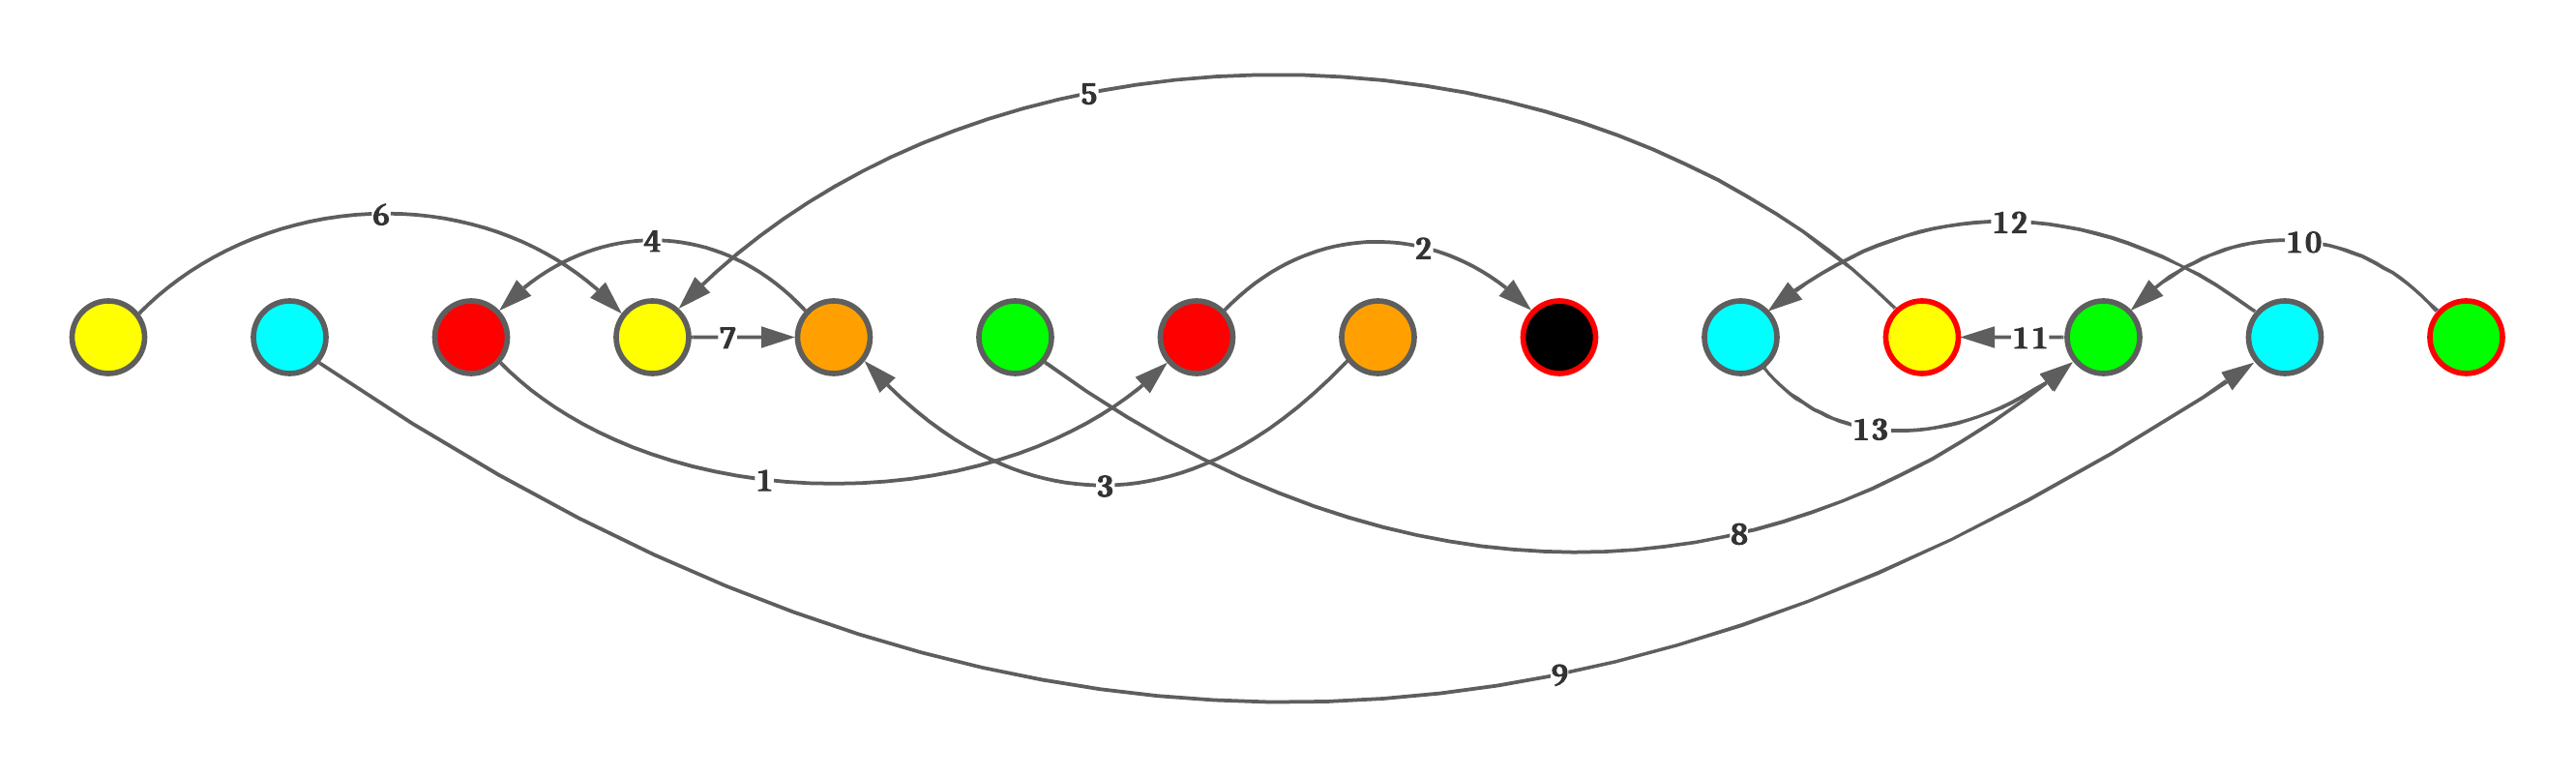
\includegraphics[width=14cm]{Images/ActSeqPic.png}
    \caption{This figure represents an activation sequence $\alpha$ with the different coloured nodes; the black, red, orange, yellow, lime and cyan nodes represent $\alpha_{\phi_0},...,\alpha_{\phi_5}$ respectively. The nodes outlined in red are the nodes contained in the sequence $(u_j)_{j=0}^k$, the function $\Gamma$ counts exactly these nodes, excluding the root node, which is the black node in this diagram.}
    \label{fig:activationsequence}
\end{figure}

We will now prove a Lemma giving a tight bound on the expected value of $\Gamma$ over random initial orderings.

\begin{lemma}\label{gamma lemma 1}
Let $\pazocal E$ be any insertion sequence of $G$, then
\[ \mathbb{E}_{\prec \in \mathcal{S}_V}[\Gamma(act(\pazocal E))] = \pazocal{O}(\log n) \]
\end{lemma}

\begin{proof}
Given some ordering $\prec$ of $V$ uniformly at random, defined by the sequence $(v_1,...,v_n)$, we can compute $\Gamma(act(\pazocal E, \prec)$ in the following way.

Create a sequence $(s_i)_{i=1}^n$ where $s_i = t$ if and only if $v_i \in \alpha_t$. Set $i_{-1}=1$. Compute $t_0 = min\{s_{t_{-1}+1},...,s_n\}$ and let $i_0=max\{i:s_i=t_0\}$. Notice that $v_{i_0} = u_0$ and $t_0 = \phi_0$. If $i_0 < n$ we can continue as follows. Compute $t_1 = min\{s_{t_{0}+1},...,s_n\}$ and let $i_1=max\{i:s_i=t_1\}$. Notice that $v_{i_1} = u_1$ and $t_1 = \phi_1$. We can continue like this forming a sequence $(i_0,...,i_k)$ until we reach $i_k = n$. We now argue that $k = \pazocal O(\log n)$.

We know that $u_0 = r$ and we expect it's position in the ordering to be $\frac{n}{2}$ since the ordering was generated uniformly at random, hence, we expect $i_0 = \frac{n}{2}$. Similarly, we expect the rightmost minimum in $\{s_{i_0+1},...,s_n\}$ to have an index of at least $i_0 + \frac{1}{2}(n - i_0)$ = $\frac{1}{2}(n+i_0)$ = $\frac{3}{4}n$, but it may be larger if there is more than one minimum. Continuing like this we can see that $\mathbb{E}[i_j] \geq n(1-2^{-1-j})$ giving us that $\mathbb{E}[i_{\log_{2}n}] \geq n-\frac{1}{2} > n - 1$ so we get that $k = \pazocal O(\log n)$.
\end{proof}

% CHAPTER 3
\section{Activation Sequences for Trees}

Fix a tree $\pazocal T=(V,E)$ with root $r$. Throughout this section we implicitly assume we are running all inputs on $\pazocal A_1$.

The activation sequences of rooted trees take a very particular form because all non-root nodes have an out-degree of exactly 1. This allows us to deduce the following Lemma, making it easy to show that the expected total recourse of $\pazocal A_1$ on trees under adversarial insertion is low.

\begin{lemma}\label{gamma lemma 2}
Let $\pazocal E$ be any insertion sequence of $\pazocal T$ and $\prec$ any initial ordering, then
\[ rec_r(\pazocal E, \prec) = \Gamma(act(\pazocal E), \prec) \]
\end{lemma}

Before proving this we must make the following simple observation.

\begin{proposition}
Let $\alpha$ be an activation sequence of $\pazocal T$. If $(x,y) \in E$, then $y$ is not activated after $x$.
\end{proposition}

\begin{proof}
Since $\pazocal T$ is a tree, there is a unique path from $x$ to $r$ and it includes $y$. Hence, when $x$ is activated (i.e. when an insertion causes $x$ to be able to reach $r$ from the first time), we know that $y$ must either be activated simultaneously or is already active.
\end{proof}

\begin{proof}[Proof of lemma 3.1]
Suppose that $rec_r(\pazocal E, \prec) > \Gamma(act(\pazocal E), \prec)$. This implies that while $x$ and $y$ are not active an edge $(x,y)$ is inserted such that $x$ is activated before $y$. Since $\pazocal T$ is a tree, $x$ can only be activated once $y$ has been activated, giving a contradiction. Hence, $rec_r(\pazocal E, \prec) \leq \Gamma(act(\pazocal E), \prec)$.

Suppose that $rec_r(\pazocal E, \prec) < \Gamma(act(\pazocal E), \prec)$. This implies that while $x$ and $y$ are not active an edge $(x,y)$ is inserted such that $y$ is activated before $x$. If such an edge is inserted, then as soon as $y$ is activated, $x$ will also be activated simultaneously, so this is not possible. Hence, $rec_r(\pazocal E, \prec) \geq \Gamma(act(\pazocal E), \prec)$.
\end{proof}

While this Lemma does not hold for DAGs in general, the second part of the proof follows from the observation we made earlier about activation sequences, so we get that $\Gamma(act(\pazocal E), \prec)$ is a lower bound on the recourse of the root for any DAG.

Now we can combine Lemma \ref{gamma lemma 1} and Lemma \ref{gamma lemma 2} to obtain the following Theorem.

\begin{theorem}
Let $\pazocal E$ be any insertion sequence of $\pazocal T$, then
\[ \mathbb{E}_{\prec \in \mathcal{S}_V}[ rec_r(\pazocal E, \prec)] = \pazocal{O}(\log n) \]
\end{theorem}

\begin{proof}
Now we can combine Lemma \ref{gamma lemma 1} and Lemma \ref{gamma lemma 2} to obtain the following equality
\[ \mathbb{E}_{\prec \in \mathcal{S}_V}[ rec_r(\pazocal E, \prec)] = \mathbb{E}_{\prec \in \mathcal{S}_V}[\Gamma(act(\pazocal E, \prec))] = \pazocal{O}(\log n) \]
\end{proof}

We can now bound the expected total recourse of $\pazocal A_1$ with a random initial ordering on trees under adversarial by $\pazocal O(n \log n)$ by applying the argument to each node individually. 

\begin{corollary}
Let $\pazocal E$ be any insertion sequence of $\pazocal T$, then
\[ \mathbb{E}_{\prec \in \mathcal{S}_V}[ rec(\pazocal E, \prec)] = \pazocal{O}(n\log n) \]
\end{corollary}

\begin{proof}
The total expected recourse is the sum of the expected recourse of every node, so by linearity of expectation we get
\[ \mathbb{E}_{\prec \in \mathcal{S}_V}[ rec(\pazocal E, \prec)] = \sum_{u \in V} \mathbb{E}_{\prec \in \mathcal{S}_V}[ rec_u(\pazocal E, \prec)] = \sum_{u \in V} \pazocal{O}(\log n) = \pazocal{O}(n\log n) \]
\end{proof}

\end{document}